\documentclass[a4paper,11pt,fleqn]{article}%fleqn pour aligner les equations à gauche
\usepackage{/home/rweye/Documents/Overleaf/Styles/Exercice}


\newcommand{\chnum}{Chapitre 5}
\newcommand{\chtitle}{Radioactivité}
\newcommand{\dtype}{Exercices Corrigés}

\begin{document}
	\maketitle
    
\section*{Exercice 1 : Types de radioactivité}
Voici une chaîne de désintégration à partir du thorium 232 :\\
\begin{tikzpicture}
\tikzstyle{etiquette}=[midway,fill=black!20]
    \node (Th232) at (-1,0) {\ce{^{232}_{90}Th}};
    \node (Ra228) at (3.5,0) {\ce{^{4}_{2}He + ^{228}_{88}Ra}};
    \draw[->] (Th232) -- (Ra228) node[etiquette]{$\alpha$};
    \node (Ac228) at (8,0) {\ce{^{228}_{89}Ac + ^{0}_{-1}e-}};
    \draw[->] (Ra228) -- (Ac228) node[etiquette]{$\beta ^-$};
    \node (Th228) at (8,-2) {\ce{^{228}_{90}Th + ^{0}_{-1}e-}};
    \draw[->] (Ac228) -- (Th228) node[etiquette]{$\beta ^-$};
    \node (Ra*) at (3.5,-2) {\ce{^{224}_{88}Ra^* + ^{4}_{2}He}};
    \draw[->] (Th228) -- (Ra*) node[etiquette]{$\alpha$};
    \node (Ra224) at (-1,-2) {\ce{\gamma} + \ce{^{224}_{88}Ra}};
    \draw[->] (Ra*) -- (Ra224) node[etiquette]{$\gamma$};
    \node (Rn220) at (-1,-4) {\ce{^{4}_{2}He + ^{220}_{86}Rn}};
    \draw[->] (Ra224) -- (Rn220) node[etiquette]{$\alpha$};
    \node (At) at (3.5,-4) {\ce{^{0}_{1}e+ + ^{220}_{85}At^*}};
    \draw[->] (Rn220) -- (At) node[etiquette]{$\beta ^+$};
    \node (At220) at (8,-4) {\ce{^{220}_{85}At + \gamma}};
    \draw[->] (At) --(At220) node[etiquette]{$\gamma$};
\end{tikzpicture}\\
Identifier à chaque étape le type de radioactivité.

\section*{Exercice 2 : Équation radioactive}
\begin{enumerate}
    \item Compléter les équations suivantes en précisant la particule $p$ et le noyau fils \ce{^A_ZX}.
    \begin{multicols}{2}
    \begin{enumerate}
        \item (\ce{\beta +}) \ce{^{15}_{8}O -> ^{15}_6C + ^{0}_{1}e+}
        \item (\ce{\gamma}) \ce{^{234}_{91}Pa^* -> ^{234}_{91}Pa + \gamma}
        \item (\ce{\beta -}) \ce{^{14}_{6}C -> ^{14}_7N + ^{0}_{-1}e-}
        \item (\ce{\gamma}) \ce{^{20}_{9}F^* -> ^{20}_{9}F + \gamma}
        \item (\ce{\beta -}) \ce{^{3}_{1}H -> ^{3}_{2}He + ^{0}_{-1}e-}
        \item (\ce{\alpha}) \ce{^{212}_{84}Po -> ^{208}_{82}Pb + ^4_2He}
        \item (\ce{\alpha}) \ce{^{172}_{79}Au -> ^{168}_{77}Ir + ^4_2He}
        \item (\ce{\beta +}) \ce{^{201}_{86}Rn -> ^{201}_{85}At + ^{0}_{1}e+}
    \end{enumerate}
    \end{multicols}
    \item Préciser les grandeurs conservées lors de ces désintégrations.\\
    Pour toutes les désintégrations on retrouve le même nombre de nucléons de chaque coté de l'équation.
    \end{enumerate}
    
\section*{Exercice 3 : Désintégration}
On considère l'équation suivante :
$$\ce{^{165}_{59}Pr -> ^{165}_{60}Nd + ^0_{-1}e-}$$
\begin{enumerate}
    \item Identifier le type de radioactivité et la particule émise.\\
    Il s'agit de la radioactivité de type $\beta ^-$, la particule émise est un électron.
\end{enumerate}
On considère maintenant l'équation de réaction suivante :
$$\ce{^A_ZX -> ^{168}_{62}Sm + ^4_2He}$$
\begin{enumerate}[resume]
    \item Identifier le type de radioactivité.\\
    Il s'agit de la radioactivité de type $\alpha$.
    \item Déterminer la composition du noyau radioactif avant sa désintégration et à quel élément il correspond.\\
    Avant désintégration le noyau contenait : 172 nucléons : 64 protons et 108 neutrons. Il s'agissant d'un noyau de Gadolinium (Gd).
\end{enumerate}

\section*{Exercice 4 : Activité radioactive}
Un échantillon de roche contenant du cobalt 59, bombardé artificiellement par des neutrons, contient dès lors \num{57E17} noyaux de cobalt 60. Au bout de 2 min, il n'en reste plus que \num{23E16}.\\
Déterminer l'activité radioactive de cette roche.\\
$A=\dfrac{dN}{dt}$, on peut ici écrire que pour nos noyaux de cobalt 60 : \\
$A_{\ce{^{60}Co}} = \dfrac{(\num{57E17} - \num{23E16})}{2\times 60} = \num{4,6E16}$ \unit{\becquerel}.

\section*{Exercice 5 : Vallée de la stabilité}
Le diagramme (N,Z) de Segrè représente l'ensemble des isotopes connus. On retrouve en rouge les isotopes stables, mais également les isotopes radioactifs en jaune et en bleu sur le schéma ci-dessous.\\
\begin{tabular}{ccccccm{4cm}}
    \cellcolor{blue!25} \ce{^{15}_5B}&\cellcolor{blue!25}\ce{^{16}_6C}&\cellcolor{blue!25}\ce{^{17}_7N}&\cellcolor{red!25}\ce{^{18}_8O}&\cellcolor{red!25}\ce{^{19}_9F}&\cellcolor{red!25}\ce{^{19}_10Ne}&\multirow{2}{*}{\huge \ce{^{14}_7N}}\\
    \cellcolor{blue!25}\ce{^{14}_5B}&\cellcolor{blue!25}\ce{^{15}_6C}&\cellcolor{blue!25}\ce{^{16}_7N}&\cellcolor{red!25}\ce{^{17}_8O}&\cellcolor{orange!25}\ce{^{18}_9F}&\cellcolor{orange!25}\ce{^{19}_10Ne}&\\
    
    \cellcolor{blue!25}\ce{^{13}_5B}&\cellcolor{blue!25}\ce{^{14}_6C}&\cellcolor{red!25}\ce{^{15}_7N}&\cellcolor{red!25}\ce{^{16}_8O}&\multicolumn{3}{c}{\textbf{Masse du noyau :} \SI{14,0067}{u}}\\
    
    \cellcolor{blue!25}\ce{^{12}_5B}&\cellcolor{red!25}\ce{^{13}_6C}&\cellcolor{red!25}\ce{^{14}_7N}&\cellcolor{orange!25}\ce{^{15}_8O}&\multicolumn{3}{c}{\textbf{Abondance :} \SI{99,634}{\percent}}\\
    
    \cellcolor{red!25}\ce{^{11}_5B}&\cellcolor{red!25}\ce{^{12}_6C}&\cellcolor{orange!25}\ce{^{13}_7N}&\cellcolor{orange!25}\ce{^{14}_8O}&\multicolumn{3}{c}{\textbf{Demi-vie :} stable}\\
    \cellcolor{red!25}\ce{^{10}_5B}&\cellcolor{orange!25}\ce{^{11}_6C}&\cellcolor{orange!25}\ce{^{12}_7N}&\cellcolor{orange!25}\ce{^{13}_8O}&\multicolumn{3}{c}{\textbf{Décroissance(s) :} noyau stable}\\
\end{tabular}

\begin{enumerate}
    \item Définir le terme isotope
    \item Donner la composition du noyau de chaque isotope de l'azote
    \item En analysant leur structure, identifier quelle particule est en excès dans chacun de ces isotopes.
    \item En déduire le type de radioactivité associée.
    \item Expliquer le fait que les isotopes d'azote 14 et 15 représentent près de 100 \% des atomes d'azote présents sur Terre.
\end{enumerate}

\section*{Exercice 6 : Radiographie au phosphore}
Un patient reçoit \SI{30}{ng} de phosphore 32 radioactif de type $\beta ^{-}$. Les émissions $\gamma$ émises par les noyaux fils du phosphore 32 permettent d'effectuer une radiographie.
\begin{enumerate}
    \item Écrire l'équation de désexcitation du noyau fils.
    \item Déterminer le nombre de noyaux injectés dans le patient.
    \item Déterminer la date à laquelle 99 \% des noyaux se sont désintégrés.    
\end{enumerate}
\textbf{Données :}
\begin{itemize}
    \item \textbf{Masse molaire du phosphore :} M(\ce{^{32}P}) = \SI{32,0}{\gram\per\mole}
    \item \textbf{Temps de demi-vie du phosphore 32 :} $t_{1/2}$(\ce{^{32}P}) = \SI{14,26}{j}
    \item \textbf{Constante d'Avogadro :} $N_A$ = \SI{6,02E23}{\per\mole}
\end{itemize}

\section*{Exercice 7 : Identification de roches}
Des roches radioactives ont été retrouvées dans un laboratoire. Après des analyses sur leur radioactivité, la décroissance radioactive de chacune de ces roches a été représentée ci-dessous :\\
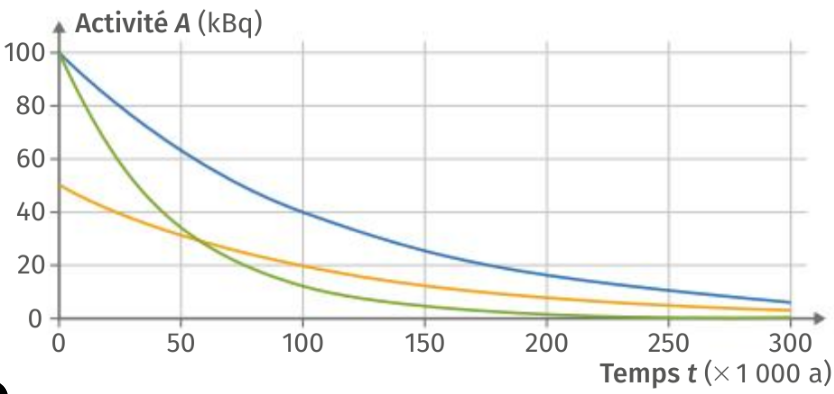
\includegraphics[scale=.5]{Ressources/TSPE_C15_Exercices_Fig1.png}
\begin{enumerate}
    \item Définir l'activité radioactive d'un échantillon.
    \item Établir la relation entre l'activité et le nombre de noyaux radioactifs présents dans l'échantillon.
    \item Identifier la nature des noyaux radioactifs présnets dans chacune de ces roches.
\end{enumerate}
\textbf{Données :}
\begin{itemize}
    \item \textbf{Temps de demi-vie :} $t_{1/2}$(\ce{^{230}Th}) = \SI{75E3}{a}
    \item $t_{1/2}$(\ce{^{202}Pb}) = \SI{53E3}{a}
    \item $t_{1/2}$(\ce{^{231}Pa}) = \SI{33E3}{a}
    \item $t_{1/2}$(\ce{^{233}U}) = \SI{159E3}{a}
\end{itemize}

\section*{Exercice 8 : Âge de la Terre}
La datation à l'uranium-plomb permet de déterminer assez précisément l'âge de la Terre, le plomb étant le produit final stable de la désintégration de l'uranium 238. Si l'on mesure la quantité de plomb 206 dans un échantillon de roche, en considérant qu'il n'y en avait pas initialement, on peut déterminer l'âge du minéral.\\
On s'intéresse à un échantillon de roche dont l'âge correspond à celui de la Terre. la courbe de décroissance radioactive théorique de cette roche est fournie dans le document 2. Le nombre de noyaux de plomb mesuré dans la roche à la date $t_{Terre}$, notée $N_{Pb}(t_{Terre})$, est égale à \num{2,5E12}.
\begin{enumerate}
    \item Indiquer le nombre initial $N_U(t_0)$ de noyaux d'uranium.
    \item Définir et déterminer graphiquement le temps de demi-vie $t_{1/2}$.
    \item Exprimer le nombre de noyaux d'uranium 239 au cours du temps.
    \item Établie la relation entre le nombre de noyaux d'uranium 238 au moment de la formation de la roche, $N_U(t_0)$, $N_U(t_{Terre})$ et $N_{Pb}(t_{Terre})$.
    \item Calculer le nombre $N_U(t_{Terre})$ de noyaux d'uraniumm et déterminer l'âge de la Terre.
\end{enumerate}
\end{document}
